\documentclass[xcolor=dvipsnames]{beamer}

% =====================================================
% CONFIGURACIÓN DEL TEMA Y ESTILO
% =====================================================
\usetheme{Madrid}
\usecolortheme{beaver}

% Colores personalizados
\definecolor{UniBlue}{RGB}{0,73,144}
\definecolor{UniRed}{RGB}{214,39,40}
\definecolor{UniGreen}{RGB}{44,162,44}
\definecolor{UniOrange}{RGB}{255,127,14}

\setbeamercolor{palette primary}{bg=UniBlue,fg=white}
\setbeamercolor{palette secondary}{bg=UniBlue!70,fg=white}
\setbeamercolor{palette tertiary}{bg=UniBlue!50,fg=white}
\setbeamercolor{frametitle}{bg=UniBlue,fg=white}

% =====================================================
% PAQUETES NECESARIOS
% =====================================================
\usepackage[utf8]{inputenc}
\usepackage[spanish]{babel}
\usepackage{amsmath,amsfonts,amssymb}
\usepackage{graphicx}
\usepackage{booktabs}
\usepackage{listings}
\usepackage{xcolor}
\usepackage{tikz}
\usepackage{pgfplots}
\usepackage{multirow}
\usepackage{array}
\usepackage{url}
\usepackage{hyperref}

% Configuración para código
\lstset{
    language=Python,
    basicstyle=\footnotesize\ttfamily,
    keywordstyle=\color{blue},
    commentstyle=\color{gray},
    stringstyle=\color{red},
    breaklines=true,
    showstringspaces=false,
    frame=single,
    backgroundcolor=\color{gray!10}
}

% =====================================================
% INFORMACIÓN DEL DOCUMENTO
% =====================================================
\title[SensorArray Lissajous]{Sistema de Detección y Análisis de Curvas de Lissajous}
\subtitle{Arreglo de Sensores con ESP32 y Fototransistores}
\author[Juan J.]{Juan J.}
\institute[Universidad]{Proyecto de Investigación Universitaria}
\date{\today}

% Logo (si tienes uno)
% \logo{\includegraphics[height=0.5cm]{logo.png}}

\begin{document}

% =====================================================
% DIAPOSITIVA DE TÍTULO
% =====================================================
\begin{frame}
    \begin{center}
        \vspace{0.5cm}
        \textcolor{UniBlue}{\Large \textbf{SensorArray for Laser Lissajous Curves}}
        
        \vspace{0.3cm}
        \textcolor{gray}{ESP32 + MicroPython + 5 Fototransistores OP598}
        
        \vspace{0.5cm}
        \begin{minipage}{0.8\textwidth}
            \centering
            \textit{Detección y análisis de movimiento láser usando un arreglo de sensores distribuidos espacialmente}
        \end{minipage}
    \end{center}
\end{frame}

% =====================================================
% TABLA DE CONTENIDOS
% =====================================================
\begin{frame}
    \frametitle{Índice}
    \tableofcontents
\end{frame}

% =====================================================
% SECCIÓN 1: INTRODUCCIÓN
% =====================================================
\section{Introducción}

\begin{frame}
    \frametitle{Motivación del Proyecto}
    \begin{columns}
        \begin{column}{0.6\textwidth}
            \begin{itemize}
                \item<1-> \textbf{Objetivo:} Desarrollar un sistema capaz de detectar y analizar patrones de movimiento láser
                \item<2-> \textbf{Aplicaciones:}
                \begin{itemize}
                    \item Análisis de vibraciones mecánicas
                    \item Detección de patrones geométricos (Lissajous)
                \end{itemize}
            \end{itemize}
        \end{column}
        \begin{column}{0.4\textwidth}
            \begin{center}
                \only<1>{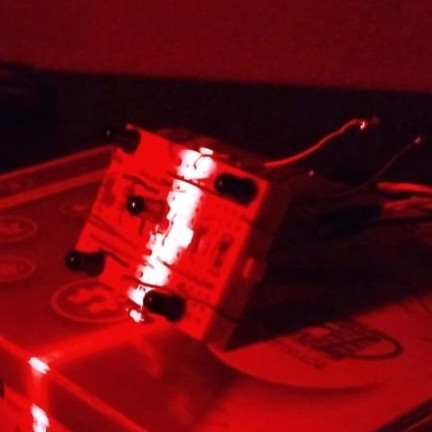
\includegraphics[width=\textwidth]{../assets/torcido.jpeg}}
                \only<2>{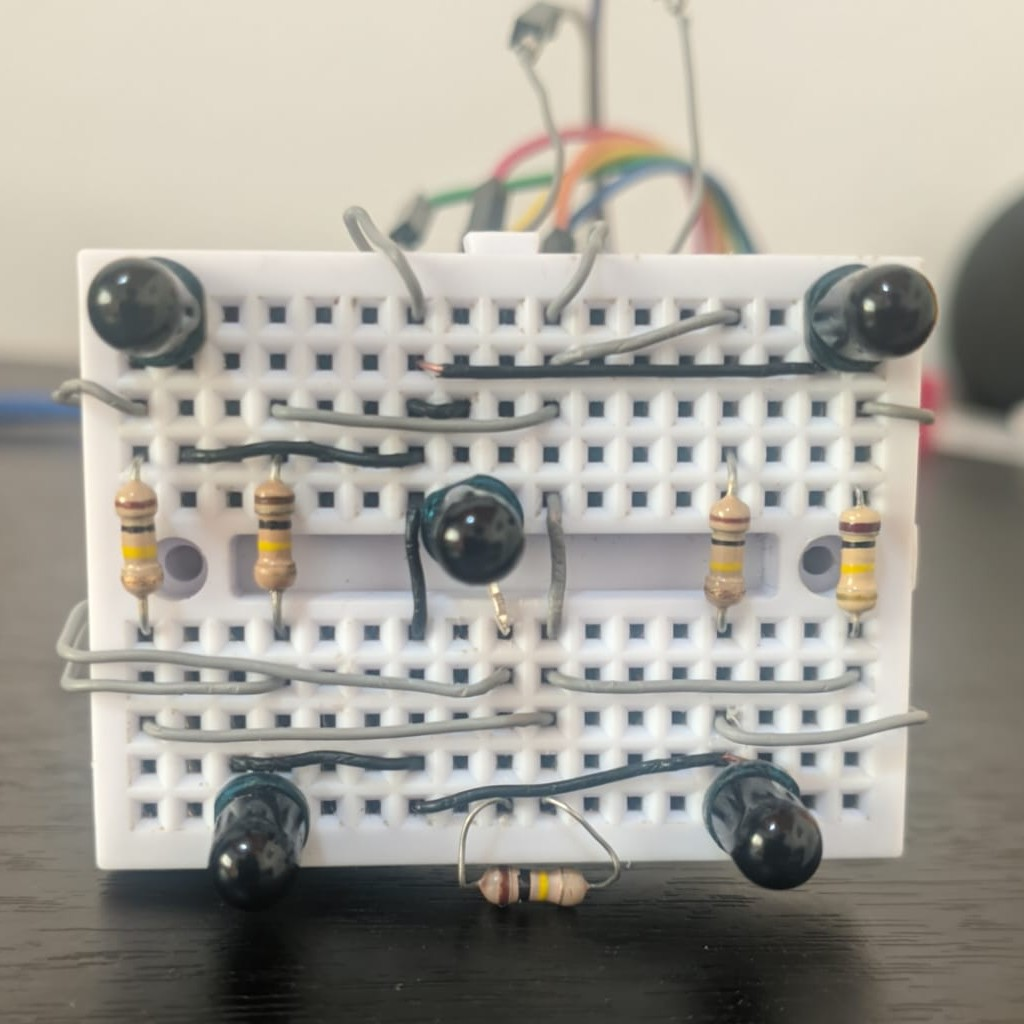
\includegraphics[width=\textwidth]{../assets/plano.jpeg}}
            \end{center}
        \end{column}
    \end{columns}
\end{frame}

% =====================================================
% SECCIÓN 2: DISEÑO DEL SISTEMA
% =====================================================
\section{Diseño del Sistema}

\begin{frame}
    \frametitle{Arquitectura General}
    \begin{center}
        \begin{tikzpicture}[
            % Aumentando distancia entre nodos
            node distance=3cm,
            % Reduciendo ancho de los bloques
            block/.style={rectangle, draw, fill=blue!20, text width=2.2cm, text centered, rounded corners},
            line/.style={draw, ->, thick}
        ]
            \node [block] (laser) {Fuente Láser\\635nm};
            \node [block, right of=laser, xshift=0.5cm] (sensors) {Arreglo de\\5 Sensores};
            \node [block, right of=sensors, xshift=0.5cm] (esp32) {ESP32\\MicroPython};
            \node [block, below of=esp32, yshift=0.5cm] (storage) {Almacenamiento\\CSV};
            \node [block, below of=sensors, yshift=0.5cm] (analysis) {Análisis\\Python/Jupyter};
            \node [block, left of=analysis, xshift=-0.5cm] (viz) {Visualización\\y Resultados};
            
            \path [line] (laser) -- (sensors);
            \path [line] (sensors) -- (esp32);
            \path [line] (esp32) -- (storage);
            \path [line] (storage) -- (analysis);
            \path [line] (analysis) -- (viz);
        \end{tikzpicture}
    \end{center}
    
    \vspace{0.5cm}
    \begin{itemize}
        \item \textbf{Entrada:} Láser de 635nm con movimiento controlado
        \item \textbf{Detección:} 5 fototransistores OP598 distribuidos espacialmente
        \item \textbf{Procesamiento:} ESP32 con adquisición a 10Hz
        \item \textbf{Análisis:} Python con librerías científicas
    \end{itemize}
\end{frame}

\begin{frame}
    \frametitle{Hardware: Componentes Principales}
    \begin{columns}
        \begin{column}{0.5\textwidth}
            \textbf{Lista de Componentes:}
            \begin{itemize}
                \item ESP32 DevKit v1
                \item 5× Fototransistores OP598 NPN
                \item 5× Resistencias 100k$\Omega$
                \item LED láser 635nm
                \item Protoboard y cables
            \end{itemize}
            
            \vspace{0.5cm}
            \textbf{Especificaciones Técnicas:}
            \begin{itemize}
                \item ADC 12-bit (0-4095)
                \item Rango: 0-3.3V
                \item Frecuencia: 10Hz
                \item Atenuación: 11dB
            \end{itemize}
        \end{column}
        \begin{column}{0.5\textwidth}
            \begin{center}
                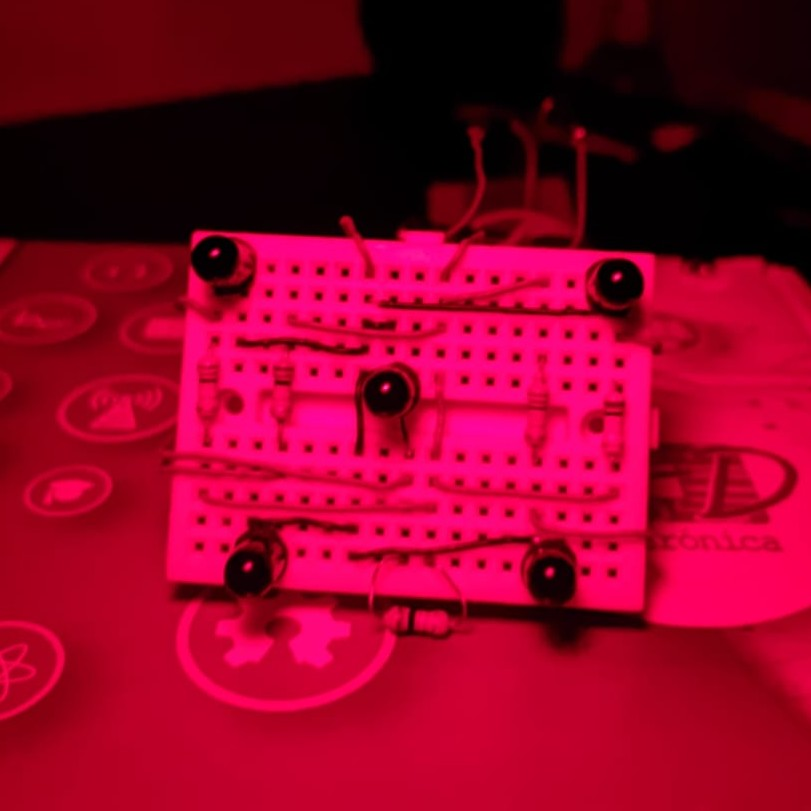
\includegraphics[width=\textwidth]{../assets/difu.jpeg}
                
                \vspace{0.3cm}
                \textit{Configuración física del sistema}
            \end{center}
        \end{column}
    \end{columns}
\end{frame}

\begin{frame}
    \frametitle{Disposición Espacial de Sensores}
    \begin{columns}
        \begin{column}{0.6\textwidth}
            \begin{center}
                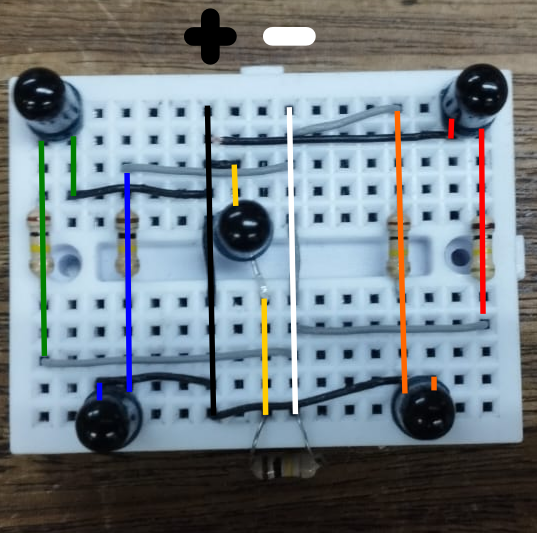
\includegraphics[width=\textwidth]{../assets/diagrama.png}
            \end{center}
        \end{column}
        \begin{column}{0.4\textwidth}
            \textbf{Coordenadas Normalizadas:}
            \begin{table}[h]
                \footnotesize
                \begin{tabular}{lcc}
                    \toprule
                    \textbf{Sensor} & \textbf{X} & \textbf{Y} \\
                    \midrule
                    Verde   & 0.0  & 1.0 \\
                    Rojo    & 1.0  & 1.0 \\
                    Amarillo& 0.47 & 0.6 \\
                    Azul    & 0.2  & 0.0 \\
                    Naranja & 0.8  & 0.0 \\
                    \bottomrule
                \end{tabular}
            \end{table}
            
        \end{column}
    \end{columns}
\end{frame}

% =====================================================
% SECCIÓN 3: IMPLEMENTACIÓN
% =====================================================
\section{Implementación}

\begin{frame}
    \frametitle{Formato de Datos}
    \textbf{Estructura CSV:}
    \begin{center}
        \begin{tabular}{|c|c|c|c|c|c|}
            \hline
            \textbf{tiempo} & \textbf{azul} & \textbf{verde} & \textbf{amarillo} & \textbf{naranja} & \textbf{rojo} \\
            \hline
            0 & 1024 & 2048 & 3072 & 1536 & 2560 \\
            100 & 1034 & 2038 & 3062 & 1546 & 2550 \\
            200 & 1044 & 2028 & 3052 & 1556 & 2540 \\
            \hline
        \end{tabular}
    \end{center}
    
    \vspace{0.5cm}
    \textbf{Características:}
    \begin{itemize}
        \item \textbf{Tiempo:} Milisegundos desde inicio de captura
        \item \textbf{Sensores:} Valores ADC (0-4095, 12-bit)
        \item \textbf{Frecuencia:} 10Hz (100ms entre muestras)
        \item \textbf{Rango útil:} 200-3500 ADC (evita saturación)
    \end{itemize}
\end{frame}

% =====================================================
% SECCIÓN 4: RESULTADOS
% =====================================================
\section{Resultados}

\begin{frame}
    \frametitle{Tipos de Patrones Detectados}
    \begin{columns}
        \begin{column}{0.5\textwidth}
            \textbf{Patrones Implementados:}
            \begin{enumerate}
                \item \textcolor{UniBlue}{\textbf{Barrido Horizontal}}
                \begin{itemize}
                    \item Movimiento lineal en X
                    \item Frecuencia: 0.5-2 Hz
                \end{itemize}
                
                \item \textcolor{UniRed}{\textbf{Barrido Vertical}}
                \begin{itemize}
                    \item Movimiento lineal en Y
                    \item Sincronización temporal
                \end{itemize}
                
                \item \textcolor{UniGreen}{\textbf{Patrones Diagonales}}
                \begin{itemize}
                    \item Movimiento esquina a esquina
                    \item Trayectorias complejas
                \end{itemize}
                
                \item \textcolor{UniOrange}{\textbf{Movimiento Aleatorio}}
                \begin{itemize}
                    \item Para calibración y pruebas
                    \item Validación de algoritmos
                \end{itemize}
            \end{enumerate}
        \end{column}
        \begin{column}{0.5\textwidth}
            \begin{center}
                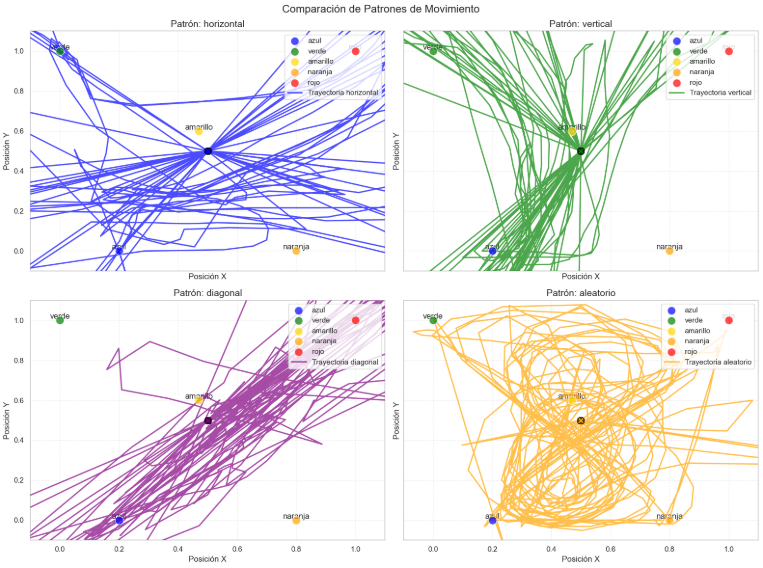
\includegraphics[width=\textwidth]{../assets/result.png}
                
                \vspace{0.3cm}
                \textit{Ejemplo de trayectoria reconstruida}
            \end{center}
        \end{column}
    \end{columns}
\end{frame}


\begin{frame}
    \frametitle{Estado Actual del Proyecto}
    \begin{alertblock}{Nota Importante}
        \textbf{Actualmente:} El sistema está validado con movimiento manual de una luz roja. La implementación de detección automática de curvas de Lissajous está en desarrollo.
    \end{alertblock}
    
    \vspace{0.5cm}
    \begin{columns}
        \begin{column}{0.5\textwidth}
            \textbf{Completado:}
            \begin{itemize}
                \item Sistema de hardware funcional
                \item Adquisición de datos estable
                \item Algoritmos de reconstrucción
            \end{itemize}
        \end{column}
        \begin{column}{0.5\textwidth}
            \textbf{En Desarrollo:}
            \begin{itemize}
                \item Detección automática de Lissajous
                \item Análisis frecuencial avanzado
                \item Interfaz de usuario
            \end{itemize}
        \end{column}
    \end{columns}
\end{frame}

% =====================================================
% SECCIÓN 5: TRABAJO FUTURO
% =====================================================
\section{Trabajo Futuro}

\begin{frame}
    \frametitle{Roadmap de Desarrollo}
    \begin{tikzpicture}[
        % Aumentando la distancia entre nodos
        node distance=3.2cm,
        phase/.style={rectangle, draw, fill=blue!20, text width=2.5cm, text centered, rounded corners, minimum height=1cm}
    ]
        \node [phase, fill=green!30] (phase1) {\textbf{Fase 1}\\Sistema Base\\(Completado)};
        \node [phase, fill=yellow!30, right of=phase1] (phase2) {\textbf{Fase 2}\\Detección Lissajous\\(En desarrollo)};
        \node [phase, fill=orange!30, right of=phase2] (phase3) {\textbf{Fase 3}\\ML \& Clasificación\\(Planeado)};
        \node [phase, fill=red!30, right of=phase3] (phase4) {\textbf{Fase 4}\\Sistema Completo\\(Futuro)};
        
        \draw[->, thick] (phase1) -- (phase2);
        \draw[->, thick] (phase2) -- (phase3);
        \draw[->, thick] (phase3) -- (phase4);
    \end{tikzpicture}
    
    \vspace{1cm}
    \textbf{Objetivos por Fase:}
    \begin{itemize}
        \item \textbf{Fase 2:} Implementar generador de Lissajous mecánico/electrónico
        \item \textbf{Fase 3:} Algoritmos de machine learning para clasificación automática
        \item \textbf{Fase 4:} Sistema completo con interfaz web y análisis en tiempo real
    \end{itemize}
\end{frame}

\end{document}
